% \chapter{Trabalhos Relacionados}
\chapter{Trabalhos relacionados}

\label{chapter:relacionados}

Existem diversas abordagens para otimizar as percepções recebidas por um agente, isto é, garantir que todas as informações coletadas pelos sensores sejam utilizadas da melhor maneira possível. Diversos artigos sobre o assunto, com diferentes abordagens, são publicados todos os anos. Para definir os trabalhos relacionados apresentados nessa seção, foram utilizados diversos termos de busca, uma vez que os termos ilusão e alucinação podem não necessariamente se aplicarem às percepções da mesma maneira definida neste trabalho.

Nos mecanismos de busca Google Scholar e Scopus foram realizadas pesquisas que associam agentes inteligentes a percepções inválidas, anomalias ou ilusões e alucinações, além de termos auxiliares como aprendizado e otimização. As buscas aconteceram ao longo do desenvolvimento do trabalho, e diversas \textit{strings} de busca foram utilizadas e combinadas. Conforme encontraram-se os artigos, suas introduções foram verificadas para averiguar se o conteúdo realmente estava relacionado ao processo de revisão de percepções. Depois disso foi realizada uma leitura inicial dos trabalhos selecionados, e os quatro mais adequados foram escolhidos para um estudo mais profundo.

Os artigos apresentados nas Seções \ref{van2011} e \ref{diab2019} implementam modelos para tratar de percepções em ambientes onde é possível receber percepções que não são totalmente confiáveis, semelhante ao conceito de anomalia definido no Capítulo \ref{conceitos-fundamentais}. Os artigos das Seções \ref{pangercic2010} e \ref{kim2017} são trabalhos relacionados a outros campos de estudo de percepção, mas que precisam resolver problemas relacionados a percepções imperfeitas. A maneira como esses artigos se conectam ao modelo proposto no trabalho atual está descrita em mais detalhes nas seções seguintes.

\section{Scalable perception for BDI-agents embodied in virtual environments \cite{van2011scalable}}

\label{van2011}
Ambientes virtuais como jogos, simulações e treinamentos exigem cada vez mais complexidade dos agentes com os quais os participantes interagem. A arquitetura BDI (\textit{belief-desire-intension}) provê a complexidade necessária para que os agentes virtuais desempenhem as tarefas avançadas necessárias. Porém, agentes BDI tradicionais possuem uma interface direta com o ambiente, enquanto os agentes dos jogos normalmente possuem um conjunto de sensores limitados para realizar suas percepções. O problema é que agentes BDI não possuem um mecanismo padrão para controlar seus sensores, decidindo quais percepções receber. Dessa maneira, o agente pode facilmente ficar sobrecarregado de informação. Para resolver esse problema, os autores desse trabalho criaram um \textit{framework} que fornece habilidades sensoriais e e atenção perceptiva para agentes BDI incorporados em um ambiente virtual, funcionando como um \textit{middleware} que atua entre o modelo cognitivo do agente e o ambiente.

Nesse \textit{framework} (representado na figura \ref{fig:bdiPerceptionModel}) toda informação do ambiente é representada pelo modelo de informação chamado \textit{Environment Object Model} (Modelo de Objeto de Ambiente) ou EOM. Objetos são definidos por classes e características, e existe uma hierarquia de objetos para agregar semântica. O \textit{middleware} é dividido entre a interface física e a interface cognitiva. A função da interface física é interagir com o ambiente para formar símbolos. Para tal, o processador sensorial primeiro recebe uma lista de possíveis percepções, que respeita filtros predeterminados implementados nos sensores. Após isso, esse processador determina se o agente está interessado nas informações recebidas, através do \textit{Interest Subscription Manager} (gerenciador de inscrição de interesse). Estes símbolos são passados para o agente na foma de percepções, que alteram os objetivos do agente. Os novos objetivos, por sua vez, são repassados para o sistema de atenção, que atualiza os interesses do agente no gerenciador de inscrição de interesse. A comunicação entre a interface física e a interface cognitiva é realizada através de mensagens, e há interfaces para que o \textit{middleware} possa se comunicar com o ambiente e com o agente, de maneira a mantê-lo independente de domínio. 

\begin{figure}[h!]
    \centering
    \caption{\textit{Framework} de percepção baseado em EOM.}
    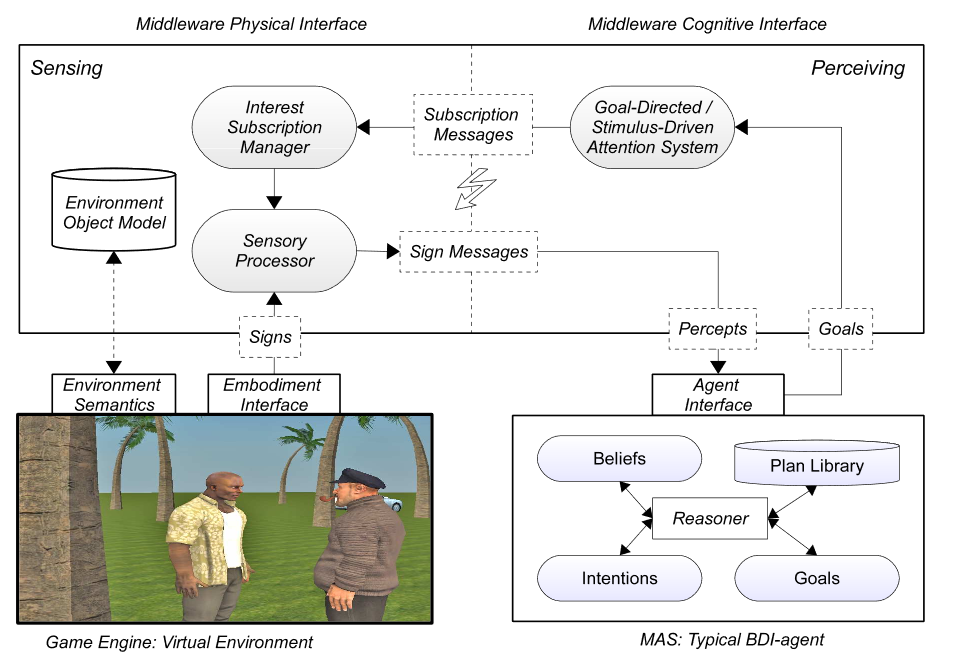
\includegraphics[width=\textwidth]{images/bdiPerceptionModel.png}
    \legend{Fonte: Scalable perception for BDI-agents embodied in virtual environments \cite{van2011scalable}.}
    \label{fig:bdiPerceptionModel}
\end{figure}

Para avaliar o modelo proposto, foram realizados dois experimentos. O primeiro consistiu no uso de sensores físicos em um teste de estresse, tanto em um sistema que utilizava o framework quando em um que não o utilizava. As percepções recebidas pelos agentes continham cinco atributos cada, sendo que a quantidade de entidades percebidas aumentava gradativamente. Cinco baterias de testes foram conduzidas para cada agente. O segundo experimento consistiu na implementação de um sistema multiagente (SMA) de agentes BDI baseado em Java e utilizando uma engine Prolog para realizar o raciocínio, e os mesmos testes do primeiro experimento foram realizados.

Esse modelo, que é capaz de decidir que tipo de percepções o agente deseja perceber de acordo com seus interesses, se assemelha ao HAIL porque muda dinamicamente ao longo do tempo, conforme as percepções são processadas. Além disso, ele possui um elemento de percepção ativa, pois o conjunto de percepções recebidas de maneira direta e massiva do ambiente é filtrado pelo processador de sensores.


\section{PMK — a knowledge processing framework for autonomous robotics perception and manipulation \cite{Diab_2019}}

\label{diab2019}
As tarefas executadas por robôs vêm se tornando cada vez mais complexas. Para realizar essas tarefas, os robôs precisam passar por uma etapa de planejamento, na qual decidem quais ações tomar baseados no estado atual do ambiente ao seu redor. Alguns dos mecanismos clássicos de planejamento utilizam a Linguagem de Definição de Domínio de Planejamento (\textit{Planning Domain Definition Language} ou PDDL) para descrever o ambiente no qual o agente está inserido. O problema é que essa abordagem assume um mundo fechado, i.e., que todos os fatos sobre o mundo são conhecidos, caso contrário o planejador pode falhar. Com essa limitação, um robô não é capaz de começar uma tarefa a não ser que todos os objetos do ambiente tenham sido reconhecidos e as ações que ele deve executar tenham sido definidas. Em outras palavras, a existência de alucinações e ilusões limita o funcionamento de tais sistemas.

Para resolver esse problema em situações onde o robô precisa realizar tarefas complexas de manipulação, foram criadas abordagens de planejamento baseadas no conhecimento, que utilizam reconhecimento semântico do cenário, conhecimento a respeito do comportamento físico de objetos e raciocínio sobre as possíveis ações de manipulação.

O trabalho de Diab et al. propõem um \textit{framework} de representação de conhecimento baseado em ontologias (uma especificação formal de conhecimento) chamado PMK (\textit{Perception and Manipulation Knowledge}), apresentado na figura \ref{fig:pmk}. Esse modelo é genérico, para que possa ser utilizado em diversos domínios, e incorporado com outras ontologias. O PMK permite associar dados de percepção de baixo nível (proveniente dos sensores, na camada física do sistema) com conhecimento de alto nível (camada de raciocínio do agente).
Uma dos principais contribuições do artigo é criar um \textit{framework} que funcione como uma caixa preta para um planejador qualquer: o PMK é capaz raciocinar sobre os recursos do robô, suas restrições de ação, a viabilidade de ação e os comportamentos de manipulação. Para isso, o modelo utiliza análise situacional, avaliando a situação a situação dos objetos no ambiente com base em posicionamento espacial, acessibilidade do robô aos objetos, potencial área na qual o objeto será colocando entre outros. 

A abordagem que é proposta pelo PMK oposta ao HAIL, pois tenta mapear todas as percepções possíveis em baixo nível a priori. Dessa forma, mesmo que o agente não tenha sido projetado para tratar determinadas percepções, ele é capaz de entender o significado semântico delas através do \textit{framework}. Em outras palavras, a ideia do PMK é criar um mapa extenso para que nenhuma percepção recebida pelo agente seja uma anomalia.

\begin{figure}
    \centering
    \caption{\textit{Framework} PMK.}
    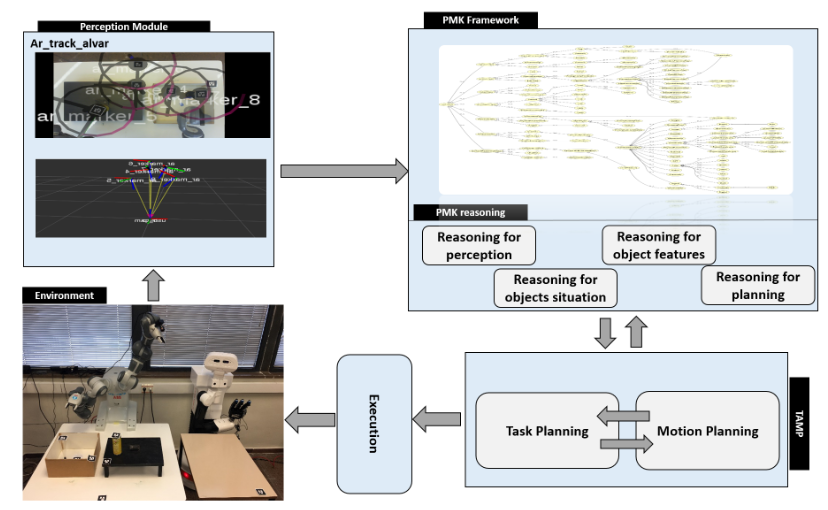
\includegraphics[width=0.9\textwidth]{images/pmk-model.png}
    \legend{Fonte: PMK - a knowledge processing framework for autonomous robotics perception and manipulation \cite{Diab_2019}.}
    \label{fig:pmk}
\end{figure}

\section{Combining perception and knowledge processing for everyday manipulation \cite{pangercic2010}}

\label{pangercic2010}
Robôs autônomos implementados para realizar tarefas de manipulação de objetos do dia a dia precisam tomar diversas decisões que requerem a combinação de percepção e processamento de conhecimento. Esse artigo de Panger et al. apresenta um sistema de programação lógica chamado K-CoPMan (\textit{Knowledge enabled Cognitive Perception for Manipulation}, ou Percepção Cognitiva Ativada pelo Conhecimento para Manipulação). Esse modelo é capaz de testar e satisfazer pré-condições de conhecimento para manipulações do dia a dia. Para isso, ele fornece ao agente o conhecimento simbólico abstrato sobre as cenas percebidas, usa conhecimento simbólico abstrato para realizar tarefas de percepção e responde a novos tipos de consultas que exigem a combinação de percepção e processamento de conhecimento.

Um dos principais mecanismos do K-CoPMan é o componente de percepção passiva. Para se tornar consciente do ambiente, o agente que utiliza tal sistema pode escanear a cena em busca de áreas de interesse, como mesas ou cadeiras, utilizar os sensores para detectar objetos. Cada objeto recebe um identificador único, para então ser guardado na base de conhecimentos, juntamente com o contexto do momento em que a percepção foi realizada. O identificador é utilizado para que mais tarde seja possível examinar mais a fundo objeto, e possivelmente classificá-lo ou categorizá-lo. Portanto, o K-CoPMan permite que agentes inteligentes estejam conscientes do ambiente ao seu redor fazendo uma varredura completa do ambiente, uma vez que utiliza tanto percepção ativa quanto passiva, e guardando as anomalias detectadas para que possam ser tratadas mais tarde por um módulo próprio (o servidor de percepção).

A abordagem desse trabalho para evitar os efeitos de percepções inválidas é similar ao PMK, mas ao invés de utilizar uma base de conhecimentos prévia para evitar que alguma percepção não possa ser tratada pelo agente, o próprio sistema cria sua base através da varredura do ambiente pela percepção passiva.

\section{Understanding human intention by connecting perception and action learning in artificial agents \cite{kim2017understanding}}

\label{kim2017}
Para desenvolver agentes capazes de realizar comportamentos complexos similares aos de seres humanos, é primeiro preciso entender como os seres humanos aprendem a perceber, pensar e agir em um mundo dinâmico. Diversos campos da inteligência artificial buscam replicar esses comportamentos, além de outros como a emoção e a cooperação. Essas habilidades parecem ser intrínsecas aos seres humanos, e tornam nossas relações mútuas únicas. Em particular, a capacidade de entender a intenção dos outros tem sido considerada a base da comunicação entre humanos. Nesse artigo, Kim, Yu e Lee propõem um modelo, chamado OA-SMTRNN (\textit{Object Augmented Supervised Multiple Timescale
Recurrent Neural Network}), para entender a intenção do usuário e responder ativamente da maneira mais adequada, através do uso de redes neurais. Para implementar o reconhecimento de intenção, são focados dois processos cognitivos, a percepção da disponibilidade de objetos e a previsão da ação humana.

Nos experimentos realizados pelos autores, diversos objetos precisaram ser percebidos pelo agente. Entretanto, alguns objetos poderiam estar sobrepostos, conforme demonstra a Figura \ref{fig:overlap}. Nesses casos, as percepções recebidas pelo agente poderiam estar incorretas. Para resolver este problema, o módulo responsável pelas ações foi implementado com a capacidade de relacionar a ação e os objetos. No artigo, é exemplificada a relação entre ``encher um copo d'água'' e ``fazer um café mocha''. Ou seja, o modelo, que foi previamente treinado, se mostrou capaz de associar a intenções como ``beber leite'' a determinadas ações (segurar um objeto, leva algo para a boca) para inferir que determinada anomalia (uma caixa de leite sobreposta por uma caneca) era uma caixa de leite.

\begin{figure}[h!]
    \centering
    \caption{Exemplo de sobreposição de imagens na percepção.}
    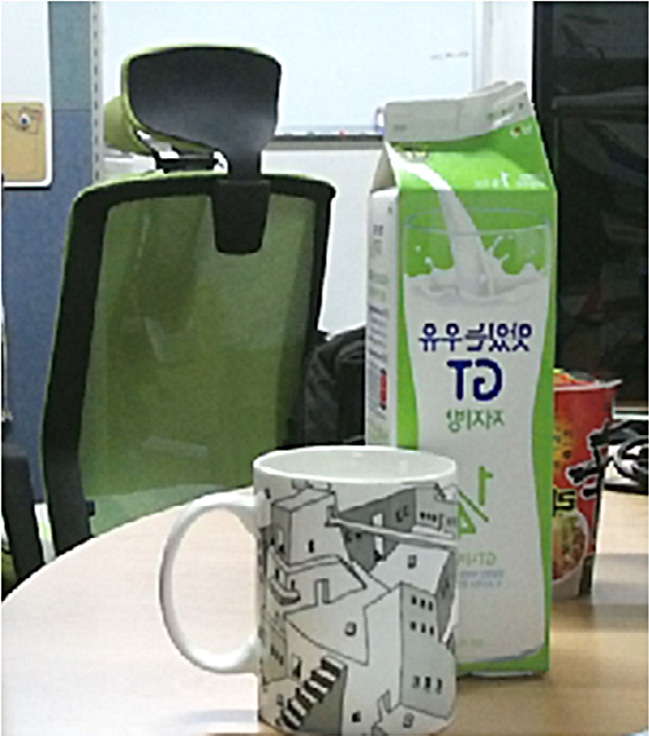
\includegraphics[width=0.5\textwidth]{images/overlap.jpg}
    \legend{Fonte: Understanding human intention by connecting perception and action learning in artificial agents \cite{kim2017understanding}.}
    \label{fig:overlap}
\end{figure}

Enquanto no modelo de revisão de percepções apresentado buscamos resolver o problema de percepção de anomalias através de uma abordagem simbólica, que classifica, trata e aprende com ilusões e alucinações, o modelo OA-SMTRNN utiliza uma abordagem conexionista, com o uso de redes neurais, para conseguir extrair semântica de percepções que seriam inicialmente inválidas para o agente. Além disso, na conclusão do trabalho é mencionado que “implementar aprendizagem de percepção-ação conectada pode desempenhar um papel importante no desenvolvimento de agentes artificiais que podem inferir a intenção humana e interagir melhor”. No HAIL, essa integração é realizada uma vez que as anomalias percebidas são utilizadas pelos módulos de planejamento automatizado para criar novos planos.

\section{Discussão}

Os quatro trabalhos que foram selecionados possuem diversas similaridades e diferenças. Para visualizar isso melhor, eles foram separados de acordo com as seguintes categorias, para então comporem o Quadro \ref{tab:relacionados}:

\begin{enumerate}
    \item Apresenta ou não um \textit{framework} genérico que pode ser aplicado em qualquer agente, independente de arquitetura;
    \item A abordagem que o trabalho utiliza para tratar percepções inválidas: limitando as percepções, de maneira que o agente realize a percepção apenas sobre as entidades que ele está pronto para tratar; definindo o ambiente, através de alguma forma de representação de conhecimento que descreve o mundo do agente para que ele possa tratar todas as percepções recebidas; ou tratar as anomalias recebidas através de algum sistema que processa as percepções inválidas recebidas;
    \item Tipos de experimentos realizados: se foram feitas simulações de software ou se foi construído um agente físico para testar o modelo;
    \item Tipos de percepções que o agente recebia: completas, no caso de ambientes simulados, ou físicas, no caso de agentes físicos;
    \item Forma de avaliação que foi utilizada para mensurar a eficácia do método proposto;
    \item Paradigma do agente (simbólico ou conexionista);
    \item Se o modelo apresenta ou não alguma ferramenta de aprendizado que utiliza ilusões e alucinações para gerar novos planos ou conhecimento.
\end{enumerate}

Através dessa classificação, é possível destacar em quais pontos nosso modelo se assemelha e diverge dos trabalhos relacionados que foram selecionados. O principal referencial do HAIL está no processo de revisão de percepções simbólico e na capacidade de permitir que qualquer arquitetura possua um processo de aprendizagem através do planejamento automatizado. Isso se reflete principalmente na forma de avaliação (tempo de processamento, como no trabalho \ref{van2011}, e também pela taxa de aprendizado do modelo) e no tipo de percepção utilizada nos experimentos (completas, pois o agente recebe a informação diretamente da simulação, mas sem semântica atrelada e sem contexto de aplicação). Além disso, três dos quatro trabalhos selecionados possuem um ambiente físico no mundo real: os trabalhos \ref{diab2019} e \ref{pangercic2010} na forma de implementação física e o trabalho \ref{kim2017} na forma de percepção de imagens que foram extraídas de um ambiente real. Isso é um indicativo de que trabalhos futuros podem implementar nosso modelo fisicamente, em robôs, por exemplo.

\begin{landscape}

% \usepackage{colortbl}


\begin{quadro}[]
\caption{Trabalhos relacionados categorizados.}
 \makegapedcells
\begin{tabular}{|P{2.3cm} |P{2.5cm}|P{2.5cm}|P{3cm}|P{2.5cm}|P{3.5cm}|P{2.3cm}|P{2.5cm}|}
\hline

\textbf{Trabalho}       & \textbf{Framework Genérico} & \textbf{Abordagem} & \textbf{Experimentos}                 & \textbf{Tipos de Percepções}                       & \textbf{Forma de Avaliação}                        & \textbf{Paradigma} & \textbf{Ferramenta de Aprendizado} \\ \hline
OIJEN; DIGNUM, 2011     & Sim (BDI)                   & Limitar percepções & Simulação de SMA com ambiente gráfico & Completas (semântica no ambiente)                  & Tempo de processamento                             & Simbólico          & Não                                \\ \hline

DIAB et al., 2019       & Sim                         & Definir o ambiente & Implementação física                  & Física (câmeras)                                   & Corretude da tarefa executada                      & Simbólico          & Não                                \\ \hline
Pangercic et. al., 2010 & Não                         & Definir o ambiente & Implementação física                  & Física (câmeras)                                   & Corretude da tarefa executada                      & Simbólico          & Não                                \\ \hline

KIM; YU; LEE, 2017      & Não                         & Tratar anomalias   & Implementação de modelo computacional & Dataset de imagens                                 & Corretude da predição                              & Conexionista       & Sim                                \\ \hline
\textbf{HAIL (trabalho atual)}          & \textbf{Sim}                         & \textbf{Tratar anomalias}   & \textbf{Simulação de agente único}             & \textbf{Completas (aleatórias e independentes de contexto)} & \textbf{Tempo de processamento e capacidade de aprendizado} & \textbf{Simbólico}          & \textbf{Sim}                                \\ \hline
\end{tabular}
 \label{tab:relacionados}
 \legend{Fonte: Autor.}
\end{quadro}

\end{landscape}


\iffalse
\newpage
\section{SEÇÃO DE TRABALHOS RELACIONADOS (ORGANIZAÇÃO)}

Essa seção estão conteúdos ligados a pesquisa de trabalhos relacionados, mas será movida ou distribuída no artigo final.

\begin{itemize}
    \item O trabalho de John Anderson [9] propõem uma versão distribuída do simulador de agentes únicos Gensim. No artigo, Anderson discorre sobre como colocar a fonte das percepções completamente dentro do agente ou do ambiente é filosoficamente impreciso. Além disso, o autor descreve como isso também representa um problema prático, uma vez que a preparação sensorial é um elemento computacionalmente intensivo, portanto um equilíbrio deve ser encontrado.
    
    \item Para Włodzisław Duch [10], em seu trabalho sobre inteligência computacional, um dos grandes problemas atuais dessa área é seu foco em raciocínio como computação, e o uso da lógica como base do raciocínio, deixando de lado o caráter técnico de como símbolos precisam primeiro serem derivados de percepções reais. Segundo o autor, o cérebro humano é altamente especializado em análise de padrões naturais e outras técnicas que permitem o mapeamento de percepções a ações, mas apesar do grande avanço na área de inteligência computacional, sistemas projetados para resolver essas funções cognitivas de ordem inferior ainda estão muito distantes da capacidade do cérebro biológico.
    
    \item Bordeux et. al. [8] apresenta uma pipeline de percepção para agentes autônomos, propondo um processo de pré-processamento, processamento e pós-processamento utilizando filtros de percepções. filtro de agente, composto por um filtro de percepção, opcionalmente um filtro semi-reflexivo (que não será discutido por estar fora do escopo do trabalho atual) e uma lista de objetos selecionados. A ideia de guardar a lista de objetos selecionados conversa com o bloco avaliador de nosso modelo, pois guarda informações de determinadas percepções realizadas para serem mais tarde reaproveitadas para um ajuste fino.
    
    \item Em um artigo de revisão sobre arquiteturas cognitivas, Langley et. al [3] caracteriza a importância de tratar de percepções imperfeitas, e mostra que as arquiteturas podem conter elementos para tratar disso, uma vez que os sensores geralmente possuem interferências ou outros tipos de ruídos, que afetam a qualidade da percepção obtida. Segundo o autor, ambientes dinâmicos complicam ainda mais a situação, uma vez que o agente precisa rastrear alterações que ocorrem muitas vezes de maneira repentina no ambiente. A única solução que o autor propõem a isso é o “conhecimento perceptivo”, onde o agente decide sobre quais sensores utilizar, onde e quando focaliza-los e que interferências são plausíveis, se aproximando da percepção ativa.
    
    \item Mesmo em simulações virtuais, às percepções podem levar a erros por conta de sua imprecisão. Sichman [6] ilustra alguns aspectos essenciais de mecanismos de raciocínio sociais, baseado na noção de dependência social. O sistema proposto trata de um modelo de coalizões, onde agentes podem se juntar em prol de um objetivo em comum. O protocolo de formação de coalizões é formado por proposições, aceitações, recusas e mensagens de revisão. As mensagens de revisão são necessárias pois uma possível razão para um agente se recusar a participar de uma coalizão é porque o remetente tem uma crença falsa sobre suas capacidades, ou seja, acreditar que o agente pode executar uma ação, mas na realidade não pode. Isso pode acontecer pois fontes de informação, como as percepções, podem levar a erros.

    \item O trabalho de Pangercic et. al. [7] trata de percepção e processamento de conhecimento, usando como estudo de caso um robô encarregado de determinar quais objetos faltam em uma mesa durante uma refeição, através de inferências lógicas. A implementação resulta em um modelo estatístico, em que cada objeto que o robô conhece recebe uma porcentagem de chance de ser necessário. Apesar dessa alta volatilidade, os autores não tratam da possibilidade da inferência incorreta.
    
    \item Diab et. al. apresenta um framework de processamento de conhecimento para a manipulação de percepção de robôs autônomos, através de raciocínio de percepção, isto é, raciocínio relacionado às características perceptivas dos objetos no ambiente, como outros modelos também fazem, mas além disso adiciona raciocínio relacionado aos algoritmos que o sensor pode executar para extrair os recursos, aos sensores associados ao robô e as limitações físicas dos sensores. Segundo os autores, esse processo torna o robô mais inteligente e flexível. Essa flexibilidade pode ser útil para lidar com a falhas de um sensores, fornecendo alternativas, ou seja, o framework proposto tem flexibilidade para lidar com sistemas sensoriais de vários modelos.
    
\end{itemize}

\textbf{Problema abordado no artigo:} Conforme abordado pelo artigo [3], interferências ocorrem entre o processo físico de percepção e o processamento final dela, dentro do ciclo cognitivo do agente. Portanto, esse trabalho ataca essa lacuna que existe, com o objetivo de minimizar percepções incorretas ou falhas completas de percepção.

\textbf{Contribuição do artigo:} Nesse artigo é apresentado um modelo genérico para o tratamento de percepções, com o objetivo de evitar que informação potencialmente útil seja desperdiçada, criando novos planos quando o agente não está pronto para lidar com percepções que estão fora do seu planejamento inicial. Esse modelo foi construído para que possa ser acoplado a qualquer arquitetura cognitiva, independente do grau de abstração que ela implemente.

\textbf{fim da seção de organização dos trabalhos relacionados}
\fi